\documentclass[10pt]{standalone}
\input{../../tikzpic_packages.tex}

\def\pneumaticcolor{blue!20}

\begin{document}
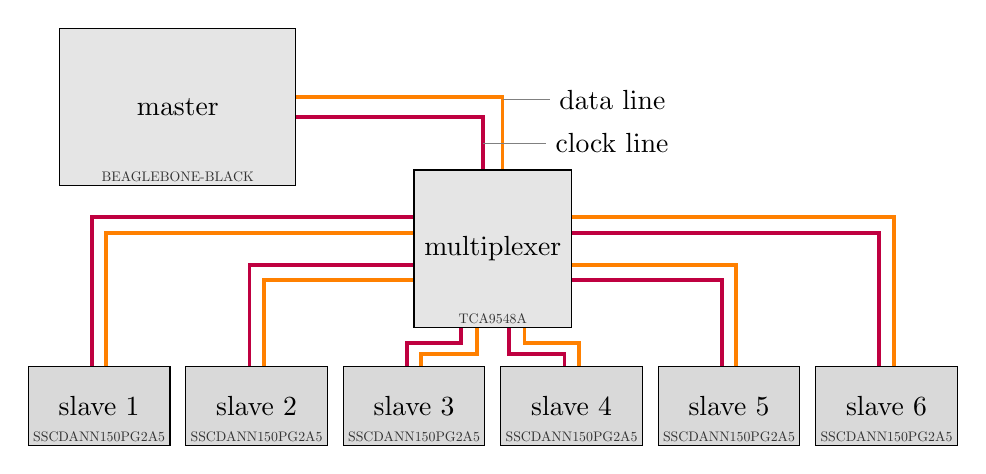
\begin{tikzpicture}[
scale = 1,
fontnode/.style={scale=.5, color=black!80},
resistor/.style={sloped, scale=.5, fill=red!50, minimum width=2cm},
life/.style={line width=.5mm, red},
gnd/.style={line width=.5mm, blue},
clk/.style={line width=.5mm, purple},
data/.style={line width=.5mm, orange},
BBB/.style={draw, fill=gray!20, minimum width=3cm, minimum height=2cm},
DSens/.style={draw, fill=gray!30, minimum height=1cm, minimum width=1.8cm},
Plex/.style={draw, fill=gray!20, minimum width=2cm, minimum height=2cm}
]

\draw (-4,1.8)node[BBB](BBB){master};
\path (BBB.south)node[fontnode, above]{BEAGLEBONE-BLACK};

\draw (0,0)node[Plex](plex){multiplexer};
\path (plex.south)node[fontnode, above]{TCA9548A};

\foreach[count=\i] \pos in {.3, .6}
	\foreach \dpos/\name in {0/c,.1/d}{
		\pgfmathsetmacro{\pp}{\pos+\dpos}
		\path (plex.north west)--(plex.south west)coordinate[pos=\pp](plex_\name\i);
		\pgfmathtruncatemacro{\ii}{\i+2}
		\path (plex.south west)--(plex.south east)coordinate[pos=\pp](plex_\name\ii);		
		\pgfmathtruncatemacro{\ii}{\i+4}
		\path (plex.south east)--(plex.north east)coordinate[pos=\pp](plex_\name\ii);		
}


\foreach[count=\i] \x in {-5, -3, -1, 1, 3, 5}{
	\path (\x, -2) node[DSens](\i){slave \i};
	\path (\i.south)node[fontnode, above]{SSCDANN150PG2A5};
%	\draw[gnd] (\i.260)--++(0,-.3)coordinate(gnd_\i);
%	\draw[life] (\i.280)--++(0,-.6)coordinate(life_\i);
}

\foreach \i in {1,2,5,6}{
	\draw[clk] (\i.100)|-(plex_c\i);
	\draw[data] (\i.80)|-(plex_d\i);}

	\draw[clk] (3.100)--++(0,.3)-|(plex_c3);
	\draw[data] (3.80)--++(0,.15)-|(plex_d3);
	\draw[clk] (4.100)--++(0,.15)-|(plex_c4);
	\draw[data] (4.80)--++(0,.3)-|(plex_d4);

\draw[data] (BBB.5)-| (plex.83)coordinate[pos=.52](data);
\draw[clk] (BBB.-5)-| (plex.97)coordinate[pos=.75](clock);

\draw[help lines] (data)--++(0:.6)node[right, black]{data line};
\draw[help lines] (clock)--++(0:.8)node[right, black]{clock line};


%\draw[gnd](gnd_6)--(gnd_1)--++(-1,0);
%\draw[life](life_6)--(life_1)--++(-1,0);



\end{tikzpicture}
\end{document}